\documentclass{article}
\usepackage[T1]{fontenc}

\usepackage{graphicx}
\usepackage{listings}
\begin{document}

\title{FOSS Lab Report}
\author{Gokul K\\[2\baselineskip]
Roll Number: 21\\[2\baselineskip]}
\date{25 January 2020}

\maketitle

\setcounter{section}{8}
\section{Shell Programming V}
\subsection{Aim}
Shell script which starts on system boot up and kills every process which uses more
than a specified amount of memory or CPU.

\subsection{Source Code}
\begin{verbatim}
#! /bin/bash

cuser="gokul"
memlimit=3.5;
cpulimit=4.0;
while ( true )
do
    echo "Script running .."
    ps -e -o  pmem=,pcpu=,pid=,user=,comm= --sort=-pmem |
    while read size cpu pid user comm
    do
        kill_mem=0
        kill_cpu=0
        if [ $user = $cuser ]
        then
            kill_mem=`echo "$size>$memlimit" | bc `
            kill_cpu=`echo "$cpu>$cpulimit" | bc `
            if [ $kill_mem = "1" ]
            then
                echo " process with PID $pid killed "
                kill $pid
            elif [ $kill_cpu = "1" ]
            then
                echo " process with PID $pid killed "
                kill $pid
            else
                continue
            fi
        fi
    done
    sleep 1
done

\end{verbatim}

\subsection{Output}
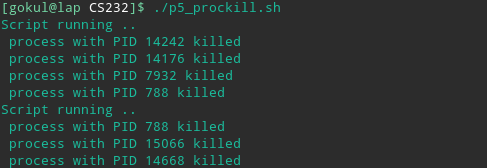
\includegraphics[width=0.9\textwidth]{img/p9/ss.png}\newline

\subsection{Result}
The above program is run on Manjaro Linux shell. Any process consuming memory greater than 3.5u and cpu greater than 4.0 and belonging to cuser were terminated.
\end{document}